
Los Discursos de odio contra mujeres, inmigrantes y muchos otros grupos es un fenómeno generalizado en la Internet. En los primeros días de la World Wide Web, algunos académicos se aventuraron a decir a que los prejuicios y el odio sería eliminado en este espacio por la disolución de identidades \cite{levy2001cyberculture, rheingold1993virtual}. Veinte años después de esta hipótesis, podemos
decir que no ha sido el caso. La prevalencia del racismo en la ``World White Web'' se ha estudiado en una serie de trabajos \cite{adams2005white, kettrey2014staking}, como así también la misoginia en el mundo virtual \cite{filipovic2007blogging, mantilla2013gendertrolling}.

El discurso racista y sexista es una constante en las redes sociales, pero los picos se documentan después de eventos ``detonantes'', como asesinatos con motivos religiosos o políticos \cite{burnap2015cyber}. Las empresas de redes sociales están preocupadas por esto y toman acciones en su contra; sin embargo, la mayoría de los esfuerzos todavía necesitan la intervención humana, lo que hace que esta tarea sea muy costosa. Reducir la intervención humana es vital para tener herramientas efectivas para evitar la escalada del discurso de odio.


En este capítulo daremos una introducción a este problema, que a su vez trataremos en los capítulos subsiguientes. Definiremos el discurso de odio y haremos una breve reseña de este fenómeno desde un marco legal, a la vez que haremos un repaso del trabajo previo. Comentaremos parte de nuestro trabajo en \citet{atalaya_tass2018} como parte de la competencia hatEval\cite{hateval2019semeval}, a la vez que marcaremos algunos problemas actuales en los enfoques actuales del discurso discriminatorio.

\section{Trabajo previo}

La detección del discurso del odio es una tarea de clasificación de oraciones bastante relacionada con el análisis de sentimientos y ha sido estudiada para varias redes sociales \cite{thelwall2008social, pak2010twitter, saleem2017web}. Con respecto a la detección de contenido que incita al odio, \citet{greevy2004classifying} usó bolsas de palabras y SVM para detectar contenido racista en páginas web. Siguiendo un enfoque similar, \citet{warner2012detecting} usó unigrams y clusters Brown con SVM para detectar mensajes antisemitas en Twitter.

\citet{waseem2016hateful} anotó un corpus y usó n-gramas de caracteres para detectar comentarios de odio, y \citet{badjatiya2017deep} usó el mismo conjunto de datos para entrenar modelos de aprendizaje profundo e incrustaciones ajustadas junto con Gradient Boosted Trees. \citet {zhang2018detecting} entrenó una red neuronal profunda que combina CNN con unidades recurrentes cerradas \cite{cho2014learning}, superando a los sistemas anteriores en varios conjuntos de datos.

\citet{anzovino2018automatic} recopiló un corpus de tweets misóginos y propuso una taxonomía para distinguirlos en diferentes categorías. Los autores propusieron una serie de técnicas diferentes para clasificarlos, mostrando que enfoques simples (como el uso de modelos lineales junto con n-gramas de token) logran un rendimiento competitivo en conjuntos de datos de pequeño tamaño.

En cuanto a las tareas compartidas, \citet{fersini2018overview} presentó un desafío en la detección de misoginia en Twitter, tanto en español como en inglés, mientras que \citet{fersini2018evalitaoverview} planteó un desafío similar pero en italiano e inglés. \citet{bosco2018overview} propuso un concurso de detección automática sobre publicaciones de Twitter y comentarios de Facebook, que incluía discursos de odio en general.


\section{Definición de discurso de odio}

\label{sec:hate_speech_definitions}

No existe una definición universalmente aceptada de lo que configura discurso de odio. En esta sección haremos un repaso muy breve de algunos tratados internacionales sobre la materia para intentar aproximarnos a este concepto, a la vez que también haremos un racconto de las definiciones utilizadas en trabajos dedicados a la construcción de datasets.

Un derecho que suele estar protegido por constituciones nacionales y tratados internacionales es el del derecho a la expresión. Por ejemplo, el Pacto de San José de Costa Rica (a la cual Argentina adhiere)\cite{humanos2018convencion} dice en su Artículo 13:

\begin{displayquote}[CADH, Artículo 13][]

    1. Toda persona tiene derecho a la libertad de pensamiento y de expresión.  Este derecho comprende la libertad de buscar, recibir y difundir informaciones e ideas de toda índole, sin consideración de fronteras, ya sea oralmente, por escrito o en forma impresa o artística, o por cualquier otro procedimiento de su elección.

    2. El ejercicio del derecho previsto en el inciso precedente no puede estar sujeto a previa censura sino a responsabilidades ulteriores, las que deben estar expresamente fijadas por la ley y ser necesarias para asegurar:

    a)  el respeto a los derechos o a la reputación de los demás, o

    b) la protección de la seguridad nacional, el orden público o la salud o la moral públicas.
\end{displayquote}

En Estados Unidos, la primer enmienda protege este derecho humano, mientras que en la Unión Europea, legislación similar ofrece protección a la libertad de expresión. Finalmente, la declaración universal de los derechos humanos de la ONU \todo{citation needed} menciona tanto en su preámbulo como en el artículo 19

\begin{displayquote}[Declaración Universal de los Derechos Humanos][ONU]
    Todo individuo tiene derecho a la libertad de opinión y de expresión; este derecho incluye el de no ser molestado a causa de sus opiniones, el de investigar y recibir informaciones y opiniones, y el de difundirlas, sin limitación de fronteras, por cualquier medio de expresión.
\end{displayquote}

Otro documento conocido como el Pacto Internacional de Derechos Civiles y Políticos (ICCPR por sus siglas en inglés) menciona

\begin{displayquote}[Artículo 19 de la ICCPR]
1. Nadie podrá ser molestado a causa de sus opiniones.

2. Toda persona tiene derecho a la libertad de expresión; este derecho comprende la libertad de buscar, recibir y difundir informaciones e ideas de toda índole, sin consideración de fronteras, ya sea oralmente, por escrito o en forma impresa o artística, o por cualquier otro procedimiento de su elección.

3. El ejercicio del derecho previsto en el párrafo 2 de este artículo entraña deberes y responsabilidades especiales. Por consiguiente, puede estar sujeto a ciertas restricciones, que deberán, sin embargo, estar expresamente fijadas por la ley y ser necesarias para:

a) Asegurar el respeto a los derechos o a la reputación de los demás;

b) La protección de la seguridad nacional, el orden público o la salud o la moral públicas.
\end{displayquote}

Sin embargo, y como mencionan estos dos últimos apartados, la libertad de expresión tiene un límite: el ejercicio de los derechos e igualdad ante la ley. Por ejemplo, el Artículo 1 del Pacto de San José de Costa Rica dice lo siguiente:

\begin{displayquote}[Pacto San José de Costa Rica, CADH][Artículo 1]
    1. Los Estados Partes en esta Convención se comprometen a respetar los derechos y libertades reconocidos en ella y a garantizar su libre y pleno ejercicio a toda persona que esté sujeta a su jurisdicción, sin discriminación alguna por motivos de raza, color, sexo, idioma, religión, opiniones políticas o de cualquier otra índole, origen nacional o social, posición económica, nacimiento o cualquier otra condición social.
\end{displayquote}

A su vez, la Declaración Universal de los Derechos Humanos en su Artículo 1:

\begin{displayquote}
    Todos los seres humanos nacen libres e iguales en dignidad y derechos y, dotados como están de razón y conciencia, deben comportarse fraternalmente los unos con los otros.
\end{displayquote}

Entonces, los Estados y otros organismos deben tomar medidas para poder asegurar el libre ejercicio de los derechos y la igualdad de todos sus miembros, aún cuando esto pueda significar una restricción en la libertad de expresión \cite{article192015}.


¿Qué es el discurso de odio entonces? Como hemos mencionado, no hay una definición universalmente aceptada. Repasemos algunas clasificaciones hechas en estos tratados para acercarnos un poco más a las características comunes que comparten.

Como vimos, el Pacto de San José de Costa Rica en su Artículo 1 habla del ejercicio de derechos sin discriminación alguna por varias razones, entre las que menciona raza, sexo, idioma, religión, política, nacionalidad, posición económica, entre otras. La Observación General 35 del Comité por la Eliminación de la Discriminación Racial de la ONU (CERD) considera que será discurso de odio, y debe ser tipificado penalmente:


\begin{displayquote}[Recomendación 35 del Comité por la Eliminación de la Discriminación Racial, CERD]

    a) Toda difusión de ideas basada en la superioridad o en el odio racial o étnico, por cualquier medio;

    b) La incitación al odio, el desprecio o la discriminación contra los miembros de un grupo por motivos de su raza, color, linaje, u origen nacional o étnico;

    c) Las amenazas o la incitación a la violencia contra personas o grupos por los motivos señalados en el apartado anterior;

    d) La expresión de insultos, burlas o calumnias contra personas o grupos, o la justificación del odio, el desprecio o la discriminación por los motivos señalados en el apartado b) anterior, cuando constituyan claramente incitación al odio o a la discriminación;

    e) La participación en organizaciones y actividades que promuevan e inciten a la discriminación racial.
\end{displayquote}

\citet{gagliardone2015countering} presenta un análisis de diversos organismos y sus definiciones de discurso de odio. En líneas generales, como se menciona en \citet{CIDH2015}, el concepto usualmente es referido a expresiones que incitan a tomar algún tipo de medida hostil contra una víctima o un grupo de personas, siendo esta perteneciente a un determinado grupo social definido por laguna característica. Dicho esto, podría delimitarse el discurso discriminatorio del discurso de odio por la componente de la promoción e instigación de la violencia; sin embargo, para los fines de este trabajo utilizaremos los términos indistintamente. Como se menciona también en \citet{CIDH2015}, aún cuando el discurso no contenga arengas ni incitaciones a cometer actos violentos, puede entenderse ese discurso como generador de un ambiente hostil y de intolerancia que termine promoviendo estos ataques físicos.


\citet{article192015} condensa muchas de estas definiciones de una manera succinta, desglosando esto en ``odio'' y ``discurso'':

\begin{displayquote}[Article 19: Hate Speech Toolkit]

    – Odio: emoción intensa e irracional de oprobio, enemistad y aborrecimiento hacia una persona o grupo de personas, por tener determinadas características protegidas (reconocidas en el derecho internacional), reales o percibidas. El “odio” es más que un mero prejuicio y debe ser discriminatorio. El odio es una muestra de un estado emocional u opinión y, por lo tanto, se diferencia de cualquier acto o acción que se haya llevado a cabo.
    – Discurso: cualquier expresión que vierta opiniones o ideas, que comparte una
    opinión o una idea interna con un público externo. Puede adoptar muchas
    formas: escrita, no-verbal, visual o artística y puede ser difundida en los
    medios, incluyendo Internet, material impreso, radio o televisión.
\end{displayquote}

%%
%%
%% Link
%% https://docs.google.com/drawings/d/149dpb2nrvmFgWZJYcrToAxO4M5n7JNQInfWd62kw3jc/edit
%%
%%

\begin{figure}[t]
    \centering
    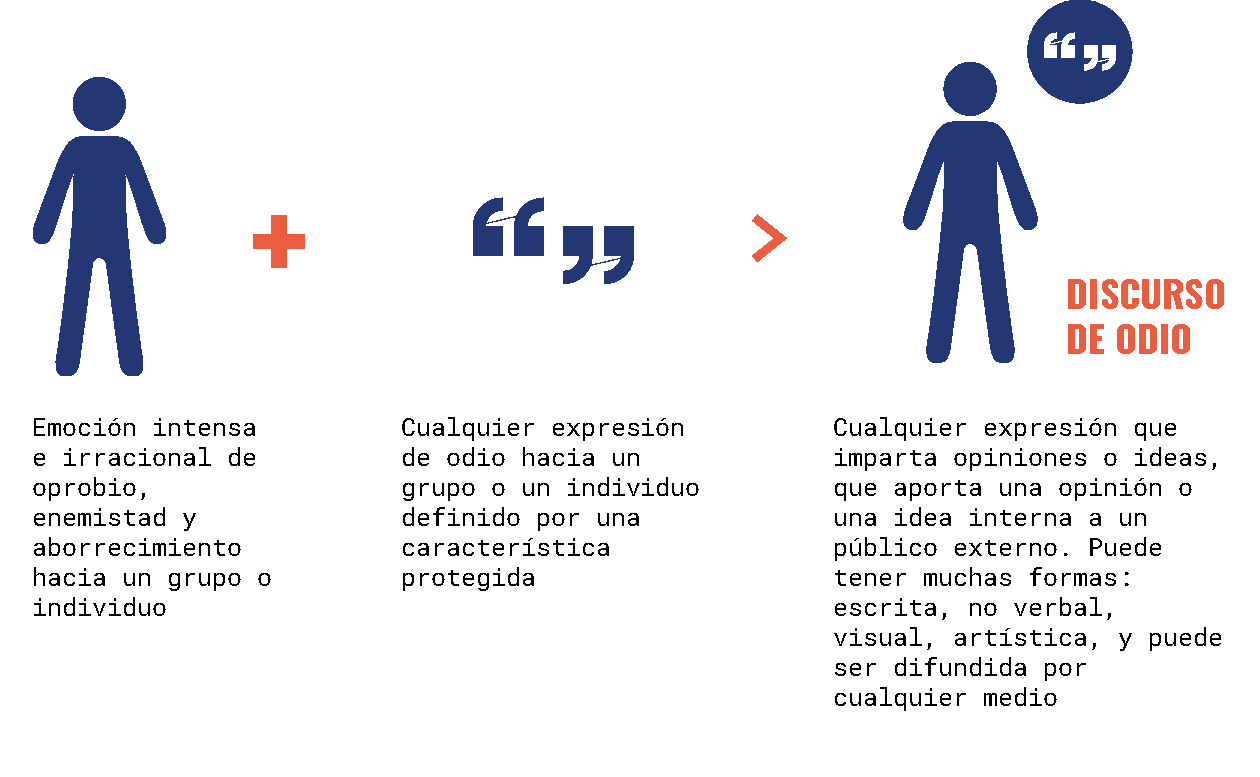
\includegraphics[width=\textwidth]{img/discurso_de_odio.pdf}
    \caption{Definición de discurso de odio de acuerdo al Toolkit de Article 19}
    \label{fig:hate_speech_definition_article_19}
\end{figure}


Entonces, puede entenderse como un discurso de cierta intensidad e irracionalidad que ataca a una persona o un grupo de personas por alguna característica históricamente vulnerada: por ser mujer, por su etnia, nacionalidad, religión, idioma, etc. La clave está en la combinación: un discurso irracional e intenso contra alguien que no posea una característica protegida no configura discurso de odio; por ejemplo, ataques a ciertas personas por ser periodistas. La figura \ref{fig:hate_speech_definition_article_19} ilustra esta definición.

No todo ataque a un individuo o una persona de algún colectivo discriminado es discurso de odio. En particular, en \citet{CIDH2015} se menciona en base al informe de la UNESCO sobre discurso de odio \citet{gagliardone2015countering} que:

\begin{displayquote}[]
    (...) el discurso de odio no puede abarcar ideas amplias y abstractas, tales como las visiones e ideologías políticas, la fe o las creencias personales. Tampoco se refiere simplemente a un insulto, expresión injuriosa o provocadora respecto de una persona. Así definido, el discurso de odio puede ser manipulado fácilmente para abarcar expresiones que puedan ser consideradas ofensivas por otras personas, particularmente por quienes están en el poder, lo que conduce a la indebida aplicación de la ley para restringir las expresiones críticas y disidentes. Asimismo, el discurso de odio tiene que distinguirse de aquellos “crímenes de odio” que se basan en conductas expresivas, como las amenazas y la violencia sexual, y que se encuentran fuera de cualquier protección del derecho a la libertad de expresión
\end{displayquote}

Como vemos, no sólamente es difusa la frontera fijada la característica sobre qué es discurso de odio o insultos, sino que incluso también es difícil definir qué característica es protegida o no. En el siguiente capítulo hablaremos más de esto al relatar cuáles fueron usadas a la hora de anotar nuestro dataset.

Si bien, como mencionamos, en cierta legislación se diferencia entre discurso discriminatorio y discurso de odio, para los fines de este trabajo utilizaremos ambas acepciones indistintamente. Cuando haya un llamado o una incitación a la violencia o algún tipo de represalia se hará explícita esta cuestión.


\section{Datasets}

En esta sección haremos un recuento de los conjuntos de datos para la detección de lenguaje odioso.
\citet{nobata2016abusive} fue uno de los primeros datasets => mencionar sus criterios, y su experimento (muy interesante) de Turkers vs anotadores in-house

% \begin{table*}
%     \centering
%     \begin{tabular*}

%     \end{tabular*}
% \end{table*}

\citet{gao2018detecting}

\subsection{Criterios de anotación}

\begin{table*}[t]
    \centering
    \begin{tabular}{p{0.20\linewidth}  p{0.80\linewidth}}
        \textbf{Hate Speech} & Language which attacks or demeans a group based on race, ethnic origin, religion, disability, gender, age, disability,
        or sexual orientation/gender identity. Some examples:
        \begin{itemize}
            \item The JEWZ are Market Manipulators Hate them freaking Jews !! To bad Hitler did not finish them off !!!
            \item  I hate the mall because there are too many unemployed apefricans and mudsharks.
            \item 300 missiles are cool! Love to see um launched into TelAviv! Kill all the gays there!
            \item EGYPTIANS ARE DESCENDED FROM APES AND PIGS. NUKE EGYPT NOW Ah me tu se ku sh
        \end{itemize} \\

        \hline

        \textbf{Derogatory} & Language which attacks an individual or a group, but which is not hate speech. Some examples:
        \begin{itemize}
            \item All you perverts (other than me) who posted today, needs to leave the O Board. Dfasdfdasfadfs
            \item yikes...another republiCUNT weighs in....
        \end{itemize} \\

        \hline

        \textbf{Profanity} & Language which contains sexual remarks or profanity. Some examples:

        \begin{itemize}
            \item T.Boone Pickens needs to take a minimum wage job in FL for a week. I guarantee he shuts the f up after that.
            \item Somebody told me that Little Debbie likes to take it up the A.\$.\$.
            \item So if the pre market is any indication Kind of like the bloody red tampons that you to suck on all day??
        \end{itemize}
         \\
    \end{tabular}
    \caption{Annotation guidelines used in \cite{nobata2016abusive}}

    \label{tab:nobata_guidelines}
\end{table*}


\subsubsection{}

\section{Método}

\subsection {Preprocesamiento}


\newcommand{\elmo}[0]{ELMo}
\newcommand{\elmomodel}[0]{\emph{LSTM-\elmo{}}}
\newcommand{\bow}[0]{BoW}
\newcommand{\boc}[0]{BoC}
\newcommand{\elmobowmodel}[0]{\emph{LSTM-\elmo{}+\bow{}}}
\newcommand{\svmmodel}[0]{$\mathrm{SVM}_0$}
\newcommand{\hateval}[0]{HatEval}
\newcommand{\semeval}[0]{SemEval-2019}
\newcommand{\fasttext}[0]{\emph{fastText}}

El preprocesamiento es crucial en las aplicaciones de PNL, especialmente cuando se trabaja con datos ruidosos generados por el usuario. Aquí, seguimos \citet{atalaya_tass2018}, definiendo dos niveles de preprocesamiento: preprocesamiento básico y orientado a sentimientos. Usamos uno u otro, dependiendo de la configuración.

El preprocesamiento básico de tweets incluye tokenización, reemplazo de identificadores, URL y correos electrónicos, y acortamiento de letras repetidas.

El preprocesamiento orientado a sentimientos incluye minúsculas, eliminación de puntuación, palabras vacías y números, lematización (usando TreeTagger \cite{schmid95}) y manejo de negación.
Para el manejo de la negación, seguimos un enfoque simple:
% \cite {das01, pang02}:
Buscamos palabras de negación y agregamos el prefijo 'NOT \_' a los siguientes tokens. Se niegan hasta tres tokens, o menos si se encuentra un token que no sea una palabra.

\section{Técnicas de clasificación}

Para capturar esta información, consideramos una representación de bolsa de caracteres que codifica recuentos de caracteres $n$ -gramas para algunos valores de $ n $. Estos vectores se calculan a partir de textos originales de tweets, sin ningún procesamiento previo. \boc {} s tienen las mismas variantes y parámetros que \bow {} s.


\subsection {Word-embeddings}

Usamos \fasttext {}, una biblioteca de incrustaciones consciente de subpalabras \cite{bojanowski16} para obtener representaciones de palabras independientes del contexto.
En lugar de usar vectores previamente entrenados disponibles públicamente, entrenamos nuestras propias incrustaciones en un conjunto de datos de $ \sim90 $ millones de tweets de varios países de habla hispana.
Preparamos dos versiones de los datos: una usando solo preprocesamiento básico y la otra usando preprocesamiento orientado a sentimientos (con la excepción de la lematización). Para estos dos conjuntos de datos, las incrustaciones de omisión de gramática se entrenaron utilizando diferentes configuraciones de parámetros, incluyendo una serie de dimensiones, tamaño de n-gramas de palabras y subpalabras, y tamaño de la ventana de contexto.

\subsection{Tweet Embeddings}
\label{sec:sif}

% Hay varias formas de usar incrustaciones de palabras para el análisis de sentimientos en tweets: los enfoques van desde el simple promedio de vectores para cada palabra en el tweet hasta el uso de arquitecturas más complejas como CNN o RNN. En este trabajo,
Se utilizaron combinaciones lineales para calcular una representación de un solo tweet.
Seguimos dos enfoques simples: promedio simple y promedio ponderado. En el segundo caso, utilizamos un esquema que se asemeja a la frecuencia inversa suave (SIF) \cite {arora17}, inspirado en la reponderación de TF-IDF.
Cada palabra $ w $ se pondera con $ \frac {a} {a + p (w)} $, donde $ p (w) $ es la palabra probabilidad unigrama y $ a $ es un hiperparámetro de suavizado.
Los valores altos de $ a $ significan más suavizado hacia el promedio simple.

% También consideramos dos opciones que afectan las incrustaciones de tweets: binarización, que ignora las repeticiones de tokens en los tweets; y normalización, que escalas dando como resultado que los vectores de tweets tengan una norma unitaria.


\subsection{Embeddings contextualizados}
\label{subsec:elmo}

Después del gran salto adelante que representó las incrustaciones de palabras independientes del contexto, llegó una nueva ola en los últimos años. En lugar de tener vectores entrenados para cada palabra, se generan representaciones dependientes del contexto para cada token dada una oración. Por ejemplo, \citet{mccann2017learned} usó un codificador LSTM profundo para traducción automática para generar vectores sensibles al contexto.

\elmo{} \cite{peters2018} es uno de estos enfoques dependientes del contexto y se basa en un modelo de lenguaje bidireccional profundo (biLM). La arquitectura del modelo de lenguaje consta de L capas de LSTM bidireccionales, además de una representación de token independiente del contexto. Por lo tanto, para cada token en una secuencia, obtenemos representaciones vectoriales de $ 2L + 1 $.
% Estas representaciones se consideran profundas ya que utilizan la salida de cada capa LSTM.
Para obtener un vector final para cada token, los autores sugieren colapsar las capas en vectores mediante una combinación lineal.

% Sea $ t_1, \ldots, t_n $ una secuencia de tokens, y sea $ h_ {k, j} $ el vector que representa la salida de la capa $ j $ cuando se consume el token $ t_k $. Entonces, el vector contextualizado para el token $ k $ es:
%
% \begin {ecuación}
% ELMo_k ^ {tarea} = \gamma ^ {tarea} \sum_ {j = 0} ^ {L} s_j h_ {k, j} \label {eq: elmo}
% \end {ecuación}

En este trabajo, usamos la implementación y los modelos entrenados previamente de \cite{che-EtAl:2018:K18-2}. El modelo español se entrenó con $L = 2 $ capas y 1024 dimensiones, y la combinación lineal se realizó utilizando un promedio simple.

\section{Resultados de clasificación}

\subsection{Análisis de Error}

\subsection{Intepretabilidad}

\section{Limitaciones}

\subsection{Problemas de anotación}

\subsection{Falta de contexto}

\subsection{Interpretabilidad y fragilidad de clasificadores}